\documentclass[dvipdfmx]{jarticle}
\usepackage{graphicx}
\newcounter{coffee}
\newcounter{bean}
\begin{document}
\begin{center}
{\large\bf コンパイラ演習課題(7)解答例}
\end{center}
\begin{list}{[\arabic{coffee}]}{\usecounter{coffee}}
    \item 
    \begin{list}{(\alph{bean})}{\usecounter{bean}}
        \item $N.val$, $L.val$, $L.d$, $B.val$
        \item 5.375\\
        \begin{center}
        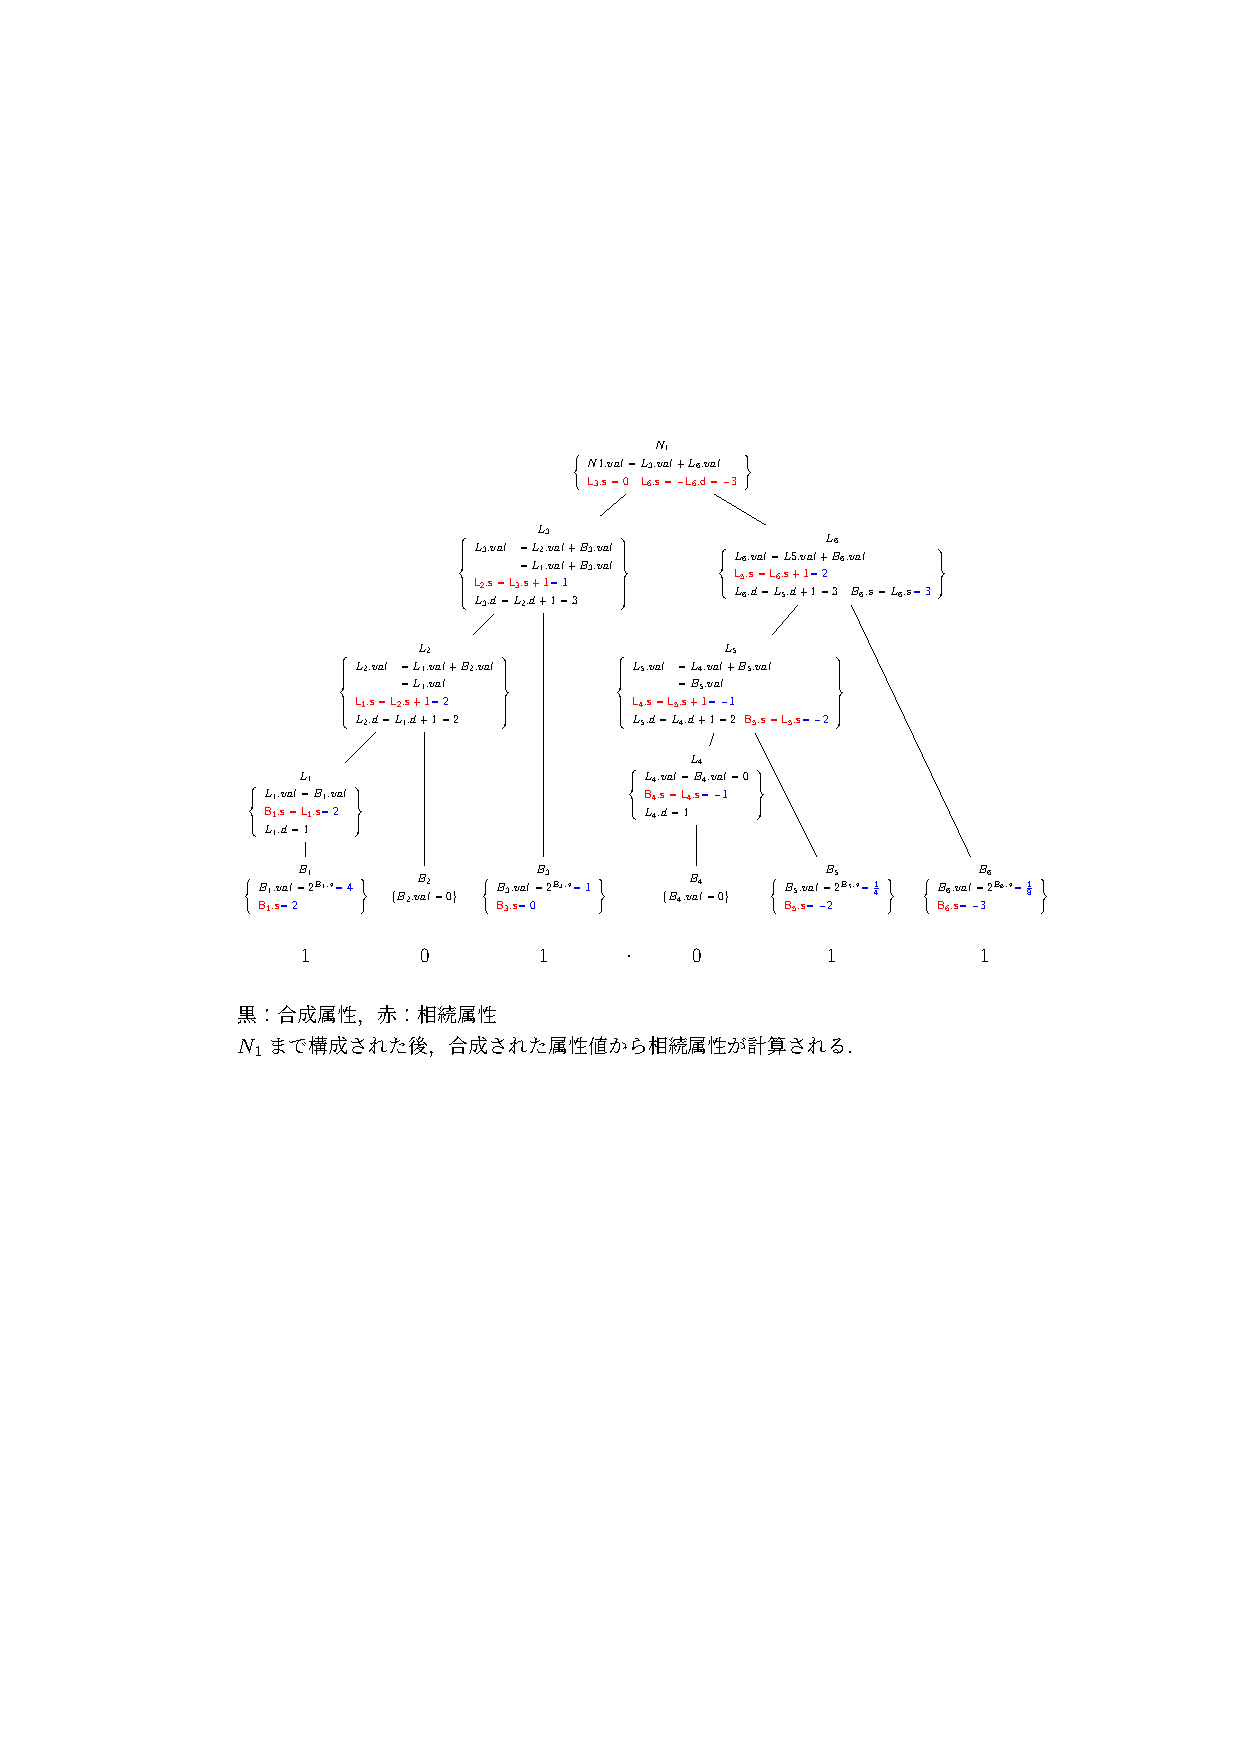
\includegraphics{attrib1-crop.pdf}
        \end{center} 
    \end{list}
    \item \begin{list}{(\alph{bean})}{\usecounter{bean}}
        \item $E.val$, $E'.b$, $T.val$ $T'.b$, $F.val$
        \item \ 各ノードにおける$(val,a,b)$として属性値を示す．\\
        \begin{center}
        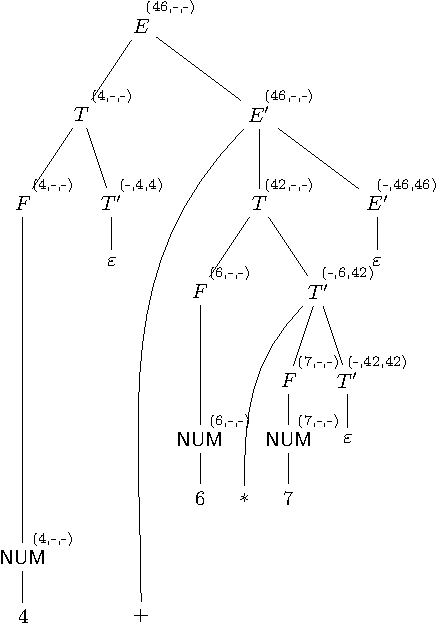
\includegraphics[height=0.4\textheight]{2atree-crop.pdf}
        \end{center} 
                \item \ 各ノードにおける$(val,a,b)$として属性値を示す．\\
        \begin{center}
        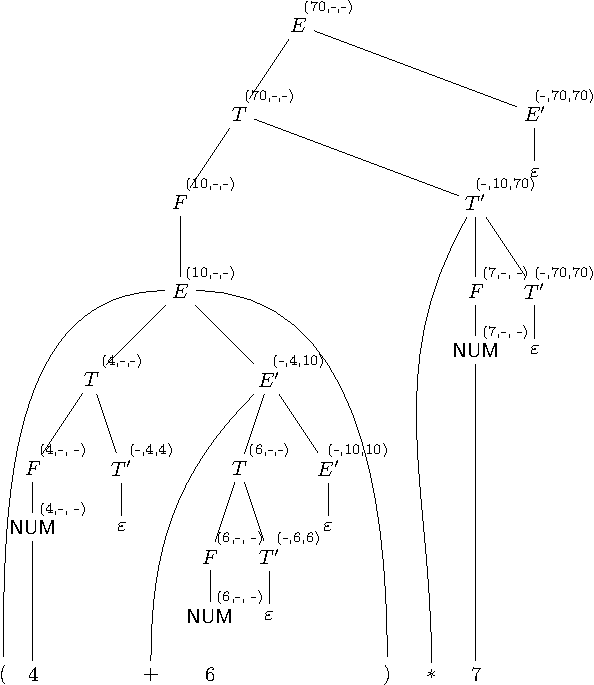
\includegraphics[height=.5\textheight]{2btree-crop.pdf}
        \end{center} 
    \end{list}
\end{list}
\end{document}